\documentclass[12pt, oneside]{article}

\usepackage[letterpaper, scale=0.89, centering]{geometry}
\usepackage{fancyhdr}
\setlength{\parindent}{0em}
\setlength{\parskip}{1em}

\pagestyle{fancy}
\fancyhf{}
\renewcommand{\headrulewidth}{0pt}
\rfoot{\href{https://creativecommons.org/licenses/by-nc-sa/2.0/}{CC BY-NC-SA 2.0} Version \today~(\thepage)}

\usepackage{amssymb,amsmath,pifont,amsfonts,comment,enumerate,enumitem}
\usepackage{currfile,xstring,hyperref,tabularx,graphicx,wasysym}
\usepackage[labelformat=empty]{caption}
\usepackage[dvipsnames,table]{xcolor}
\usepackage{multicol,multirow,array,listings,tabularx,lastpage,textcomp,booktabs}

% NOTE(joe): This environment is credit @pnpo (https://tex.stackexchange.com/a/218450)
\lstnewenvironment{algorithm}[1][] %defines the algorithm listing environment
{   
    \lstset{ %this is the stype
        mathescape=true,
        frame=tB,
        numbers=left, 
        numberstyle=\tiny,
        basicstyle=\rmfamily\scriptsize, 
        keywordstyle=\color{black}\bfseries,
        keywords={,procedure, div, for, to, input, output, return, datatype, function, in, if, else, foreach, while, begin, end, }
        numbers=left,
        xleftmargin=.04\textwidth,
        #1
    }
}
{}
\lstnewenvironment{java}[1][]
{   
    \lstset{
        language=java,
        mathescape=true,
        frame=tB,
        numbers=left, 
        numberstyle=\tiny,
        basicstyle=\ttfamily\scriptsize, 
        keywordstyle=\color{black}\bfseries,
        keywords={, int, double, for, return, if, else, while, }
        numbers=left,
        xleftmargin=.04\textwidth,
        #1
    }
}
{}

\newcommand\abs[1]{\lvert~#1~\rvert}
\newcommand{\st}{\mid}

\newcommand{\A}[0]{\texttt{A}}
\newcommand{\C}[0]{\texttt{C}}
\newcommand{\G}[0]{\texttt{G}}
\newcommand{\U}[0]{\texttt{U}}

\newcommand{\cmark}{\ding{51}}
\newcommand{\xmark}{\ding{55}}


\begin{document}
\begin{flushright}
    \StrBefore{\currfilename}{.}
\end{flushright}{\bf Definition} For $b$ an integer greater than $1$, $w$ a positive integer, 
$w'$ a positive  integer, and $x$ a real number the {\bf base $b$ fixed-width 
expansion of $x$ with integer part width $w$  and fractional part width $w'$} is
$(a_{w-1} \cdots a_1 a_0 .  c_{1} \cdots c_{w'})_{b,w,w'}$
where  $a_0, a_1, \ldots, a_{w-1}, c_1, \ldots, c_{w'}$ are nonnegative integers less than $b$ and
$$x \geq \sum_{i=0}^{w-1} a_{i} b^{i} + \sum_{j=1}^{w'}  c_{j} b^{-j} \hfill
\textrm{\qquad and \qquad}
\hfill x < \sum_{i=0}^{w-1} a_{i} b^{i} + \sum_{j=1}^{w'} c_{j} b^{-j} + b^{-w'}$$
\begin{center}
\begin{tabular}{|c|p{5in}|}
\hline
& \\
$3.75$  in fixed-width binary,& \\
integer part width $2$,&\\
 fractional part width $8$ & \\
& \\
\hline
& \\
$0.1$  in fixed-width binary, & \\
integer part width $2$, &\\
 fractional part width $8$ & \\
& \\
\hline
\end{tabular}
\end{center}
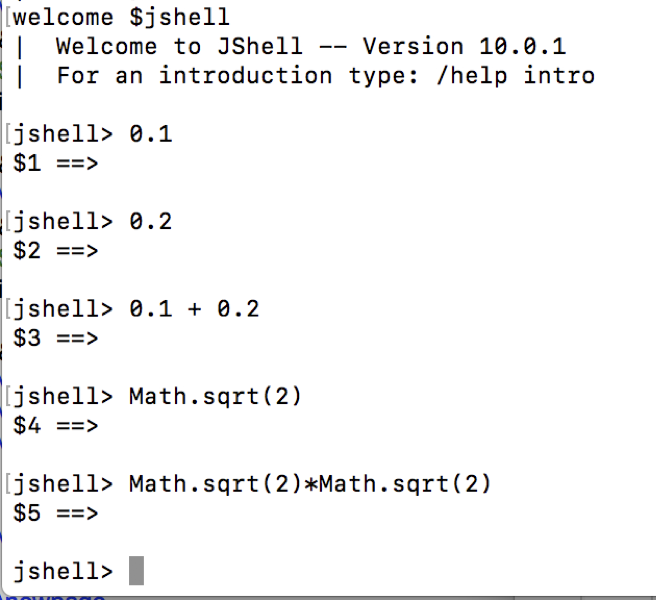
\includegraphics[width=2in]{../../resources/images/ArithmeticDemo.png}
Note: Java uses floating point, not fixed width representation, but similar rounding errors appear in both.

\end{document}